\let\negmedspace\undefined
\let\negthickspace\undefined
\documentclass[journal]{IEEEtran}
\usepackage[a5paper, margin=10mm, onecolumn]{geometry}
%\usepackage{lmodern} % Ensure lmodern is loaded for pdflatex
\usepackage{tfrupee} % Include tfrupee package

\setlength{\headheight}{1cm} % Set the height of the header box
\setlength{\headsep}{0mm}     % Set the distance between the header box and the top of the text

\usepackage{gvv-book}
\usepackage{gvv}
\usepackage{cite}
\usepackage{amsmath,amssymb,amsfonts,amsthm}
\usepackage{algorithmic}
\usepackage{graphicx}
\usepackage{textcomp}
\usepackage{xcolor}
\usepackage{txfonts}
\usepackage{listings}
\usepackage{enumitem}
\usepackage{mathtools}
\usepackage{gensymb}
\usepackage{comment}
\usepackage[breaklinks=true]{hyperref}
\usepackage{tkz-euclide} 
\usepackage{listings}
% \usepackage{gvv}                                        
\def\inputGnumericTable{}                                 
\usepackage[latin1]{inputenc}                                
\usepackage{color}                                            
\usepackage{array}                                            
\usepackage{longtable}                                       
\usepackage{calc}                                             
\usepackage{multirow}                                         
\usepackage{hhline}                                           
\usepackage{ifthen}                                           
\usepackage{lscape}
\begin{document}

\bibliographystyle{IEEEtran}
\vspace{3cm}

\title{8.4.14}
\author{EE25BTECH11011 - Navya}
% \maketitle
% \newpage
% \bigskip
{\let\newpage\relax\maketitle}

\renewcommand{\thefigure}{\theenumi}
\renewcommand{\thetable}{\theenumi}
\setlength{\intextsep}{10pt} % Space between text and floats
\textbf{Question}:\\

Let $\mathbf{P}(x_1, y_1) $ and $\mathbf{Q}(x_2, y_2)$, $ y_1 < 0, y_2 < 0 $, be the endpoints of the latus rectum of the ellipse $x^2 + 4y^2 = 4$
Then, the equations of the parabolas with latus rectum $PQ$ are
\begin{enumerate}
\begin{multicols}{2}

    \item $ x^2 + 2\sqrt{3}y = 3 + \sqrt{3} $
    \item $ x^2 - 2\sqrt{3}y = 3 + \sqrt{3} $
    \item $ x^2 + 2\sqrt{3}y = 3 - \sqrt{3} $
    \item $ x^2 - 2\sqrt{3}y = 3 - \sqrt{3} $
\end{multicols}
\end{enumerate}


\textbf{Solution}:\\
Consider the ellipse defined by the quadratic form
\begin{align}
\mathbf{x}^\top \mathbf{V} \mathbf{x} + 2 \mathbf{u}^\top \mathbf{x} + f = 0,
\end{align}

where
\begin{align}
\mathbf{V} = \begin{bmatrix} 1 & 0 \\ 0 & 4 \end{bmatrix}, \quad
\mathbf{u} = \mathbf{0}, \quad
f = -4.
\end{align}

The eigenvalues and eigenvectors of $\mathbf{V}$ are
\begin{align}
\lambda_1 = 1, \quad \mathbf{p}_1 = \begin{bmatrix} 1 \\ 0 \end{bmatrix}, \quad
\lambda_2 = 4, \quad \mathbf{p}_2 = \begin{bmatrix} 0 \\ 1 \end{bmatrix}.
\end{align}

The eccentricity $e$ of the ellipse is given by
\begin{align}
e = \sqrt{1 - \frac{\lambda_1}{\lambda_2}} = \sqrt{1 - \frac{1}{4}} = \frac{\sqrt{3}}{2}.
\end{align}

Define the vector
\begin{align}
\mathbf{n} = \sqrt{\lambda_2} \mathbf{p}_1 = 2 \begin{bmatrix} 1 \\ 0 \end{bmatrix} = \begin{bmatrix} 2 \\ 0 \end{bmatrix}.
\end{align}



The formula for $c$ is:
\begin{align}
c = \frac{ \mathbf{u}^\top \mathbf{n} \pm \sqrt{ e^2 (\mathbf{u}^\top \mathbf{n})^2 - \lambda_2 (e^2 - 1)( \|\mathbf{u}\|^2 - \lambda_2 f ) } }{ \lambda_2 e (e^2 - 1) }.
\end{align}

Since $\mathbf{u} = \mathbf{0}$, this simplifies to:
\begin{align}
c = \pm \frac{ \sqrt{ - \lambda_2 (e^2 - 1)( - \lambda_2 f ) } }{ \lambda_2 e (e^2 - 1) }.
\end{align}

Calculate the terms inside the square root:
\begin{align}
e^2 - 1 &= \frac{3}{4} - 1 = -\frac{1}{4}, \\
- \lambda_2 (e^2 - 1)( - \lambda_2 f ) &= -4 \times \left(-\frac{1}{4}\right) \times (-4 \times -4) = 16.
\end{align}

Thus,
\begin{align}
c &= \pm \frac{\sqrt{16}}{4 \times \frac{\sqrt{3}}{2} \times \left(-\frac{1}{4}\right)} = \mp \frac{2}{\sqrt{3}}
\end{align}


The focus $\mathbf{F}$ of the ellipse can be calculated as
\begin{align}
\mathbf{F} = \frac{c e^2 \mathbf{n}}{\lambda_2} = \frac{c \times \frac{3}{4} \times \begin{bmatrix} 2 \\ 0 \end{bmatrix}}{4} = \frac{3c}{8} \begin{bmatrix} 2 \\ 0 \end{bmatrix} = \frac{3c}{4} \begin{bmatrix} 1 \\ 0 \end{bmatrix}.
\end{align}

Choosing $c = \frac{2}{\sqrt{3}}$, we get
\begin{align}
\mathbf{F} = \frac{\sqrt{3}}{2} \begin{bmatrix} 1 \\ 0 \end{bmatrix}.
\end{align}

The endpoints $\mathbf{x}_1, \mathbf{x}_2$ of the latus rectum $PQ$, where $y_1, y_2 < 0$, satisfy the ellipse equation
\begin{align}
x^2 + 4 y^2 = 4.
\end{align}
Substituting $x = \sqrt{3}$, we find
\begin{align}
y = -\frac{1}{2},
\end{align}

so the endpoints are
\begin{align}
\mathbf{P} = \begin{bmatrix} \sqrt{3} \\ -\frac{1}{2} \end{bmatrix}, \quad
\mathbf{Q} = \begin{bmatrix} -\sqrt{3} \\ -\frac{1}{2} \end{bmatrix}
\end{align}

The midpoint (vertex) $\mathbf{V}$ of the latus rectum is
\begin{align}
\mathbf{V} = \frac{\mathbf{P} + \mathbf{Q}}{2} = \begin{bmatrix} 0 \\ -\frac{1}{2} \end{bmatrix}.
\end{align}

The length of the latus rectum is
\begin{align}
|\mathbf{P} - \mathbf{Q}| = 2 \sqrt{3} = 4a,
\end{align}

which gives
\begin{align}
a = \pm\frac{\sqrt{3}}{2}.
\end{align}


The parabola with vertex $\mathbf{V}$ and parameter $a$ has equation:
\begin{align}
x^2 = 4 a (y - y_0),
\end{align}

where $y_0 = -\frac{1}{2}$. Substituting $a =\pm\frac{\sqrt{3}}{2}$, we get


\textbf{Case 1:} $a = +\dfrac{\sqrt{3}}{2}$\\
\begin{align}
x^2 - 2\sqrt{3}y &= 3 + \sqrt{3}.
\end{align}

\textbf{Case 2:} $a = -\dfrac{\sqrt{3}}{2}$\\
\begin{align}
x^2 + 2\sqrt{3}y &= 3 - \sqrt{3}.
\end{align}

Hence, the equations of the required parabolas are
\begin{align}
\boxed{
x^2 - 2\sqrt{3}y = 3 + \sqrt{3}
\quad \text{and} \quad
x^2 + 2\sqrt{3}y = 3 - \sqrt{3}.
}
\end{align}

\begin{figure}[h!]
    \centering
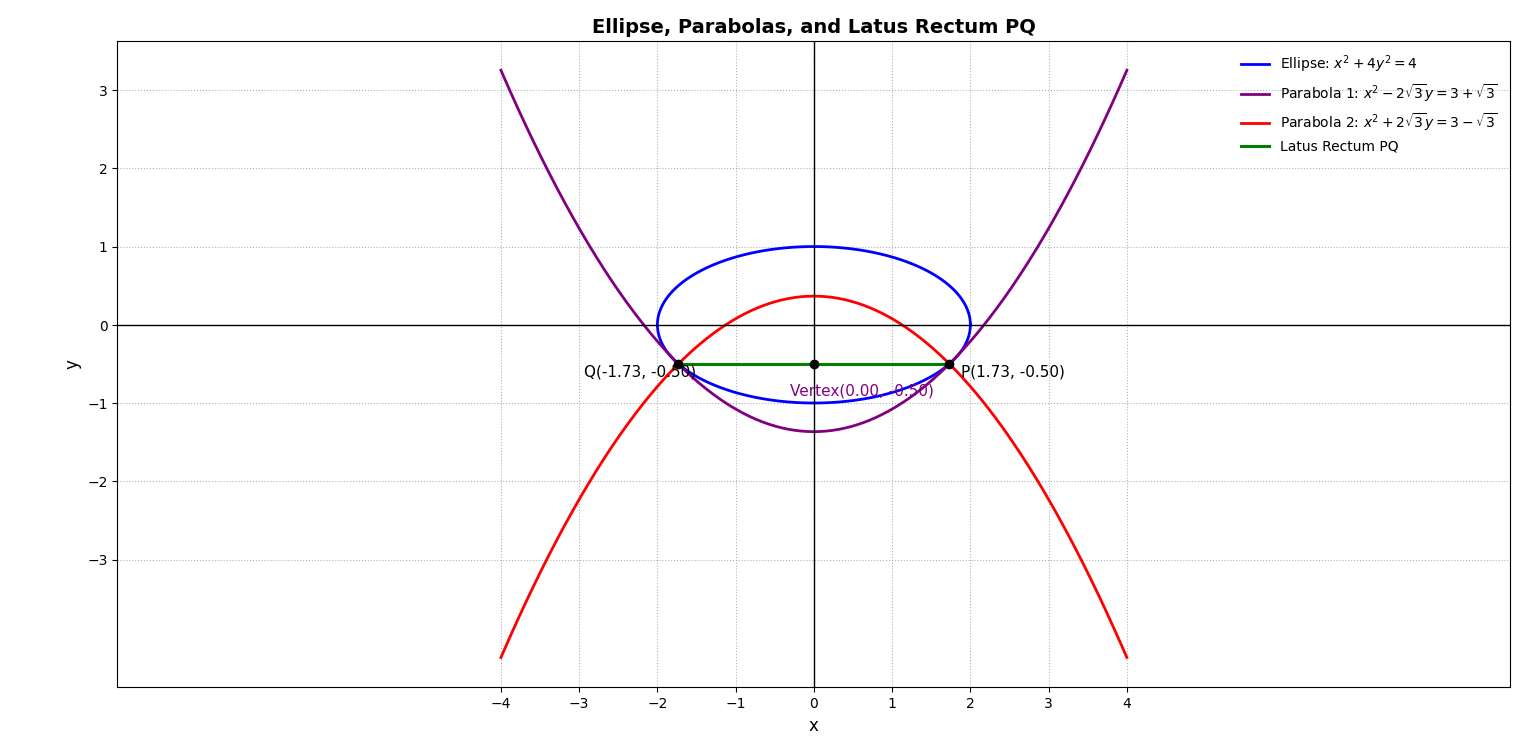
\includegraphics[width=0.8\textwidth]{figs/fig14.png}
    \label{fig:division}
\end{figure}

\end{document}
